\documentclass{article}
\usepackage{graphicx}
\usepackage{listings}
\usepackage{color}
\usepackage{tikz}
\usetikzlibrary{mindmap}  % Mindmap drawing library 
\graphicspath{{./img/}}
\begin{document}
\section{intro to robotics}
\subsection{what is robotics}
\par\noindent\rule{\textwidth}{0.4pt}
\subsubsection{Accd. RIA 1979}
\begin{itemize}
	\item reprogramable device
	\item multifunctional manipulator
	\item to move material,part,tools or specialised device
	\item using various programing methods
\end{itemize}
\subsubsection{Japanese Industrial robots association (JIRA)}
\begin{itemize}
	\item device with degrees of freedom that can be controlled
\end{itemize}
\section{Laws of robotics}
\begin{itemize}
	\item robot may not injure human
	\item obey order given by humans
	\item must protect itself complying with 1st and 2nd law
\end{itemize}
\subsection{capabilites of robots}
\begin{itemize}
	\item autonomy:perform task - based on current state - wihtout human intervention
	\item sense - plan - act
\end{itemize}
\subsection{Types of robots }
\subsubsection{according to application}
\begin{itemize}
	\item Industrial robots - industrial use
	\item service robots - domestic use
\end{itemize}
\subsubsection{based on useage and area}
\begin{itemize}
	\item manipulator
	      \begin{itemize}
		      \item Industrial robots
		      \item collabrative robots (cobots)
	      \end{itemize}
	\item mobile robots
	      \begin{itemize}
		      \item legged moblie robots
		      \item wheeled robots
	      \end{itemize}
	\item terrestrail robots - cheetah robots
	\item Aerial robots and underwater robtos
	\item Mobile manipulator
\end{itemize}


\newpage
\section{Robotics terminology}
\textbf{workspace} - volume in which end effector can reach (oreientation and position)
\textbf{Degeree of freedom} - minimum no of co ordinates needed to describe a system
\begin{itemize}
	\item \textbf{redundant manipulator}- spatial manipulator more than 6 DOF / planar with more than 3 DOF
	\item \textbf{underactuated manipulator}- spatial with less than 6 DOF / planar with less than 3 DOF
\end{itemize}
\textbf{postion} - tranlational location of something \\
\textbf{oreientation} - rotational location of something (roll, pitch,yaw) \\
\textbf {kinematics} - study of motion without regards of forces \\
\textbf{dynamcis} - study of foreces with regard of forces \\
\textbf{actuator} - provide the force for robots motion \\
\textbf{sensor} - estimate robots condition in robot's condidtion and environment \\
\textbf{Accuracy} - ability to position itself to the desired loaction with minimum error
\begin{itemize}
	\item  \textbf{accuracy} - depends on machine accuracy in construction
	\item can be improve by kinamatic calibiration
\end{itemize}
\textbf{Repeatebility} - ability to do a task repeateadly\\
\begin{itemize}
	\item depends on robot controller and mesaurement resolution
\end{itemize}
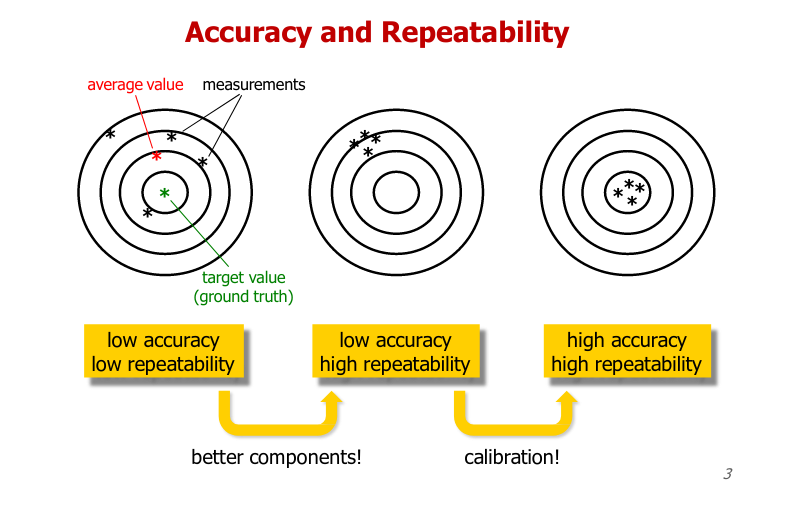
\includegraphics[width=13cm]{accuracy.png}
\newpage
\textbf{Spatial Resolution}
\begin{itemize}
	\item smallest increment of movement in which robot can divide its work
	\item depends on control resolution and mechanical inaccuracies
\end{itemize}
\textbf{stability} - maintaining output over time/temperature
\par\noindent\rule{\textwidth}{0.4pt}
\newpage

\section{Elements of robots}
\subsection{Mechanical systems}
\begin{itemize}
	\item \textbf{links} - connects the joints
	\item \textbf{Parts} - supporting structure,end effector , chasis, wheels etc
\end{itemize}
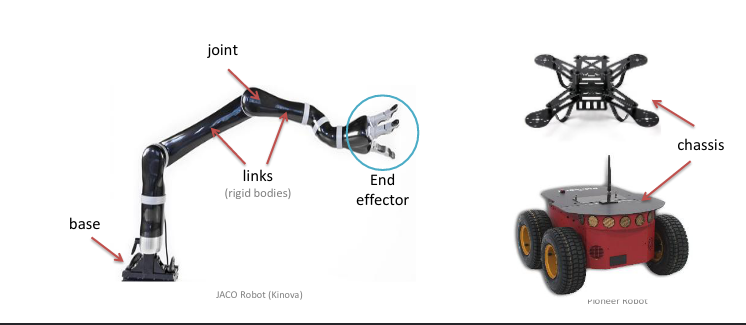
\includegraphics[width=13cm]{img/mechanicalSystem.png}
\subsection{Sensing systems}
\begin{itemize}
	\item \textbf{proprioceptive sensors}
	      \begin{itemize}
		      \item Internal state of robot
		      \item position,velocity,torque of joint
	      \end{itemize}
	\item \textbf{exteroceptive}
	      \begin{itemize}
		      \item external environment
		      \item camera,proximity
	      \end{itemize}
\end{itemize}
\subsection{Actuation systems}
\begin{itemize}
	\item Motors - electric,hydraulilc,pneumatic
	\item Algos for moot control
	\item Transmissions
\end{itemize}
\subsection{Control system}
\begin{itemize}
	\item Brain of the robots
	\item 2 levels
	      \begin{itemize}
		      \item \textbf{Low level} - Motor control
		      \item \textbf{High level} - Planning,task control, Learining
	      \end{itemize}
\end{itemize}
\section{Rigid Bodies}
Set of particle with constant realtive distance distance between any 2 particles
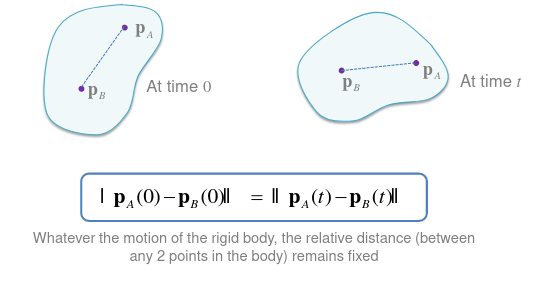
\includegraphics{img/rigidBodies.png}
\textbf{Spatial rigid bodies} - it moves in 3D
\textbf{Planar rigid bodies} - it moves in 2d
\section{Configuration of rigid bodies}
\subsection{Configuration}
\begin{itemize}
	\item complete specification of all points of  rigigd body
	\item complete specification of all points of postion and oreientation
	\item \textbf{Examples}
	      \begin{itemize}
		      \item configuration of hinge  \(\theta\)
		      \item configuration of a point in plane  $(x,y)$
		      \item confiuration of rigid body in plane $(x,y,\theta)$ \\
		            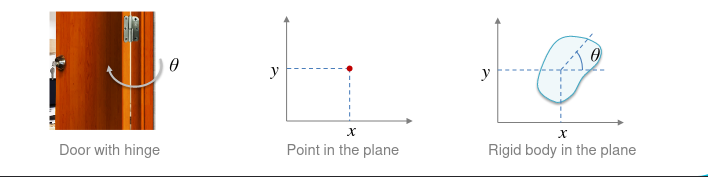
\includegraphics[width=11cm]{img/configurationRigid.png}
	      \end{itemize}
\end{itemize}
\subsection{Degrees of freedom}
\begin{itemize}
	\item minimum no of co-ordinates needed to represent the config of rigid body
	\item no of independant co-ordinates required to represent configuration
	      \begin{center}
		      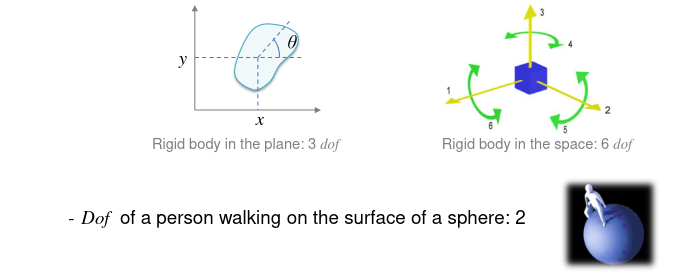
\includegraphics[width=10cm]{img/dof-rigidbody.png}
	      \end{center}
\end{itemize}
\subsection{Mecahnisms}
\begin{itemize}
	\item Closed chain mechanism
	      \begin{itemize}
		      \item the have closed loop
		      \item Examples
		            \begin{itemize}
			            \item 4 bar linkage
			            \item Parallel robots
		            \end{itemize}
	      \end{itemize}
	\item open chain mecahnism
	      \begin{itemize}
		      \item No loops
		      \item series of link and joints
	      \end{itemize}
\end{itemize}
\section{How to represent a robot}
\begin{center}
	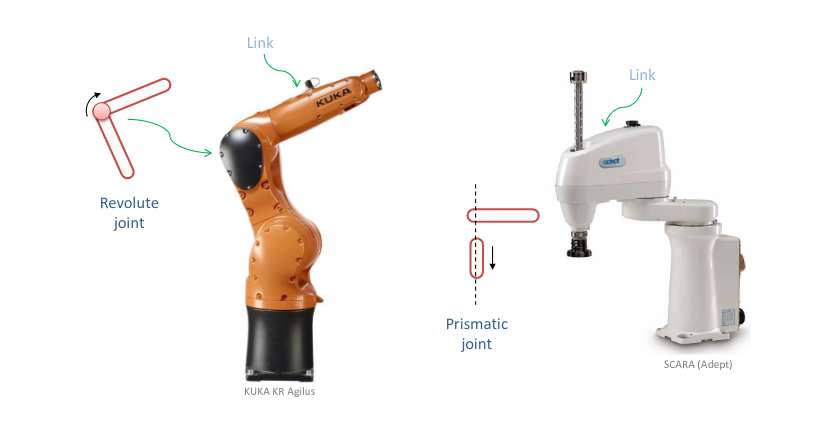
\includegraphics[width=10cm]{img/represent-robot.png}
\end{center}
\subsection{Robot configuration }
\begin{itemize}
	\item complete specification of every points in robots (position and orientation)
	\item configuration of every free link - 6 parameters
	\item every joint - 5 parameters
	\item every link - 1 parameters
	\item configuration of a complete robtot - 2 parameters
\end{itemize}
\subsection{Degrees of freedom }
\begin{itemize}
	\item minimum no of independent co-ordinates to represent a robot
	\item $dof = (\sum freedom of every link) - (independant constrains)$
	      \begin{center}
		      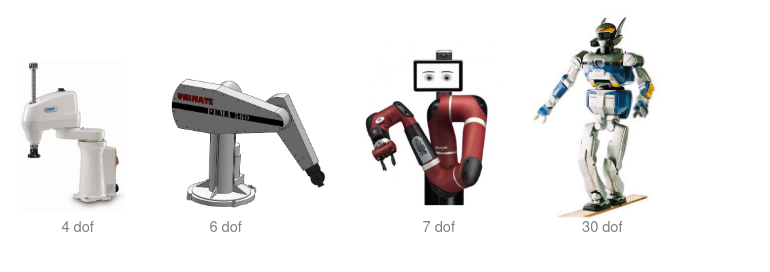
\includegraphics[width=10cm]{img/diffrent-dof.png}
	      \end{center}
\end{itemize}
\section{Joints}
\begin{itemize}
	\item they are th connection between two links
	\item \textbf{Function}
	      \begin{itemize}
		      \item constrain motion of a link with respect to each other (reduce DOF)
		      \item provide freedom for motion of link
	      \end{itemize}
	\item \textbf{DOF of joint}
	      \begin{itemize}
		      \item every independant motion that a joint allows
	      \end{itemize}
	\item In general, DOF of robot depends on number of link and joints (grubler formula)

\end{itemize}
\newpage
\subsection{Most used joints in robotics}
\subsubsection{Prismatic joint}
\begin{itemize}
	\item allows tranlational movement on a fixed axis
	\item 1 doffor motion
	\item 5 constrains to spatial motion
	      \begin{figure}[htpb]
		      \centering
		      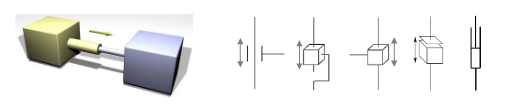
\includegraphics[width=0.8\textwidth]{prismaticjoint}
		      \caption{}
		      \label{fig:}
	      \end{figure}
\end{itemize}
\subsubsection{Revolute joint}
\begin{itemize}
	\item allows rotational movement on fixed axis
	\item 1 dof
	\item 5 constrains
	      \begin{figure}[htpb]
		      \centering
		      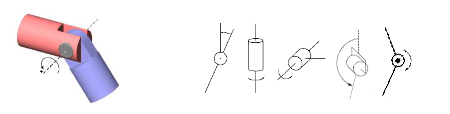
\includegraphics[width=0.8\textwidth]{revolutejoint}
		      \caption{revolutejoint}
		      \label{fig:revolutejoint}
	      \end{figure}
\end{itemize}
\newpage
\subsubsection{Helical joint }
\begin{itemize}
	\item Also known as screw
	\item allow simulataneous but dependant movement in rotational and translational axis
	\item 1 dof
	\item 5 constrains
	      \begin{figure}[htpb]
		      \centering
		      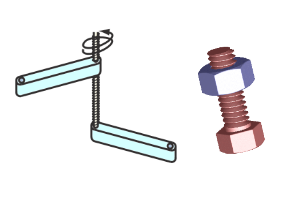
\includegraphics[width=0.4\textwidth]{helical-joint}
		      \caption{helical-joint}
		      \label{fig:helical-joint}
	      \end{figure}
\end{itemize}
\subsubsection{Cylinderical joint}
\begin{itemize}
	\item independant rotation and translational movement
	\item 2 dof
	\item 4 constrains
	      \begin{figure}[htpb]
		      \centering
		      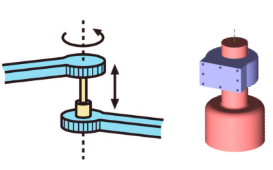
\includegraphics[width=0.3\textwidth]{cylinderical-joint}
		      \caption{cylinderical-joint}
		      \label{fig:cylinderical-joint}
	      \end{figure}
\end{itemize}
\newpage
\subsubsection{Universal joint }
\begin{itemize}
	\item  2 revolute joints with their axis are orthagonal
	\item 2 dof
	\item 4 constrains
	      \begin{figure}[htpb]
		      \centering
		      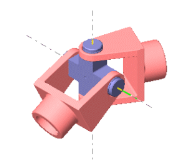
\includegraphics[width=0.2\textwidth]{universal-joint}
		      \caption{universal-joint}
		      \label{fig:universal-joint}
	      \end{figure}
\end{itemize}
\subsubsection{Spherical joint}
\begin{itemize}
	\item ball and socket joint
	\item 3 dof
	\item 3 constrains
	      \begin{figure}[htpb]
		      \centering
		      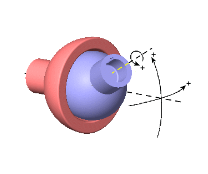
\includegraphics[width=0.3\textwidth]{spherical-joint}
		      \caption{spherical-joint}
		      \label{fig:spherical-joint}
	      \end{figure}
\end{itemize}
\newpage
\section{robots based on physical configuration}
\begin{itemize}
	\item Cartesian configuration
	\item Cylinderical configuration
	\item Polar configuration
	\item Joint-arm configuration
\end{itemize}
\subsection{Cartesian configuration}
\begin{itemize}
	\item Links are connected with linear joints
	\item example gantry robots
	\item 3 Prismatic joints
	\item commonly used for
	      \begin{itemize}
		      \item pick and place
		      \item assembly operations
		      \item handling machine tools
		      \item arc weldings
	      \end{itemize}
	      \begin{figure}[htpb]
		      \centering
		      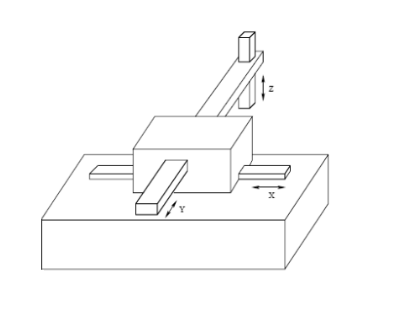
\includegraphics[width=0.4\textwidth]{cartesianRobot.png}
		      \caption{}
		      \label{fig:}
	      \end{figure}
\end{itemize}
\subsubsection{advantages}
\begin{itemize}
	\item ablity to do straight line insertions
	\item easy computation and programming
	\item most rigid structure for given length
\end{itemize}
\subsubsection{disadvantages}
\begin{itemize}
	\item require large operating volume
	\item exoposed guiding surface leads to corrosion
	\item can only reach front itself
	\item axes hard to seal
\end{itemize}
\section{Cylinderical configuration}
\begin{itemize}
	\item one rotational joint and two linear joint
	\item example versatran 600
	\item commonly used for
	      \begin{itemize}
		      \item handling die casting
		      \item assembly operations
		      \item machine tools
		      \item spot welding
	      \end{itemize}
	      \begin{figure}[htpb]
		      \centering
		      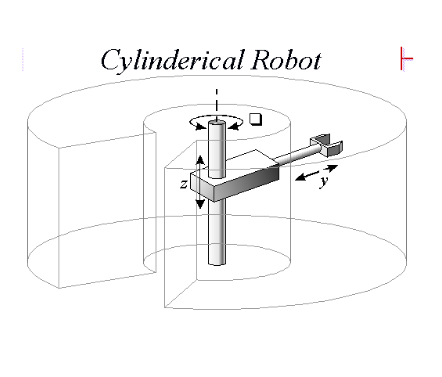
\includegraphics[width=0.3\textwidth]{CylindericalConfiguration.png}
		      \caption{}
		      \label{fig:}
	      \end{figure}
\end{itemize}
\subsection{Advantages}
\begin{itemize}
	\item can reach around itself
	\item rotaitonal axis easy to seal
	\item easy programming
	\item rigid to handle heavy loads
\end{itemize}
\subsection{Disadvantages}
\begin{itemize}
	\item cant reach above itself
	\item linear axes hard to seal
	\item wont reach around obstacles
\end{itemize}
\section{Polar/Speherical robots}
\begin{itemize}
	\item have work space of spheraical robots
	\item 2 rotary joints and one prismatics joint
	\item example Unimate 2000B
	      \begin{figure}[htpb]
		      \centering
		      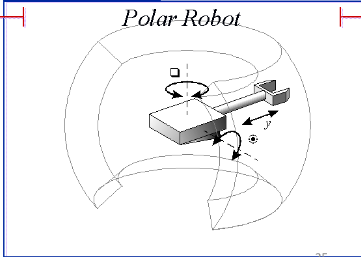
\includegraphics[width=0.3\textwidth]{polarrobots.png}
		      \caption{}
		      \label{fig:}
	      \end{figure}
	\item commonly used for
	      \begin{itemize}
		      \item die casting and fettling
		      \item handling machine tools
		      \item arc/spot welding
	      \end{itemize}
\end{itemize}
\subsection{Advantages}
\begin{itemize}
	\item large working envelope
	\item two rotational drive are sealed easily
\end{itemize}
\subsection{Disadvantages}
\begin{itemize}
	\item Complex co ordinates difficult program and visualise
	\item exposed linear drive
	\item Low accuracy
\end{itemize}
\section{Joint-arm configuration}
\begin{itemize}
	\item Combination of cylinderical and articulated joints
	\item base connected with twisting joint
	\item arm joint are rotatory
	\item Many commericial robots use this
	      \begin{figure}[htpb]
		      \centering
		      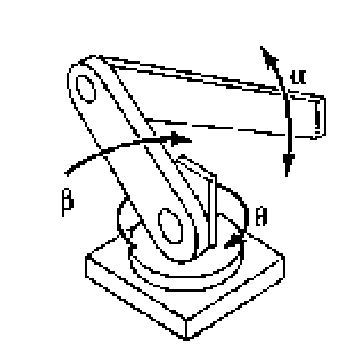
\includegraphics[width=0.2\textwidth]{jointarmConfig.png}
		      \caption{}
		      \label{fig:}
	      \end{figure}
\end{itemize}
\section{Articulated Robots}
\begin{itemize}
	\item Robots with 3 rotatory joints
	\item example T3,PUMA
	\item Commonly used for
	      \begin{itemize}
		      \item assembly operation
		      \item Welding
		      \item Weld sealing
		      \item Spray painting
		      \item die casting
	      \end{itemize}
	      \begin{figure}[htpb]
		      \centering
		      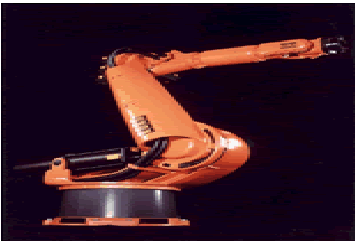
\includegraphics[width=0.3\textwidth]{articulatedRobots.png}
		      \caption{}
		      \label{fig:}
	      \end{figure}
\end{itemize}
\subsection{Advantages}
\begin{itemize}
	\item maximum flexibility
	\item any point total volume can be reached
	\item all joints can be sealed
\end{itemize}
\subsection{Disadvantages}
\begin{itemize}
	\item Extremely difficult to program visualise and controll
	\item restricted volume coverage
	\item low accuracy
\end{itemize}
\section{SCARA }
\begin{itemize}
	\item selective compliance Articulated robot arm
	\item 2 parallel robots arm
	\item commonly used for pick and place
\end{itemize}
\subsection{Advantages}
\begin{itemize}
    \item High speed 
    \item Height axis is rigid 
    \item large work area in floor space 
    \item moderately easy to program
\end{itemize}
\subsection{Disadvantages}
\begin{itemize}
    \item Limited application
    \item 2 ways to rach a point
    \item difficult to program off line
    \item highly complex arm
\end{itemize}
\end{document}


